\glsresetall
\chapter{Proposta de Virtualização e Migração de Processos para \textit{Lightweight Manycores}}
\label{chap.dev.virtualizacao}

Este trabalho de conclusão propõe-se a aumentar a independência dos processos no processador através do projeto e desenvolvimento do suporte à virtualização e migração de processos em \lws. Ambientes \cloud, nos quais o sistema de memória é de alta capacidade, usufruem da utilização de \vms para isolar duplicatas inteiras de \oss com o auxílio da virtualização a nível de instrução~\cite{sharma2016containers}. Em oposição, \lws não dispõem de centenas de GBs de memória, mas sim pequenas memórias locais. Isso associado a outras simplificações de \hardware faz com que algumas técnicas de virtualização sejam impraticáveis nesses ambientes computacionais.


Nesse contexto, visando atenuar o impacto da virtualização no sistema de memória, o presente trabalho explora um modelo de virtualização mais leve, baseado em contêineres adaptado para \lws. O \so executa os contêineres como aplicações virtuais. Sendo assim, não há a necessidade de um \os convidado, resultando em um menor impacto no sistema de memória e requisitando menor complexidade do \hardware~\cite{thalheim2018cntr, sharma2016containers}.


\section{contexto de um processo}
\mytodo{threads, memoria, syscall, comunicação, estruturas de sincronização}
\mytodo{conteinerização no nanvix}



\begin{figure}[t]
	\centering
	
	\subcaptionminipage[fig.nanvix.without-uarea]%
                   {.4\textwidth}
                   {\os sem isolamento.}
                   {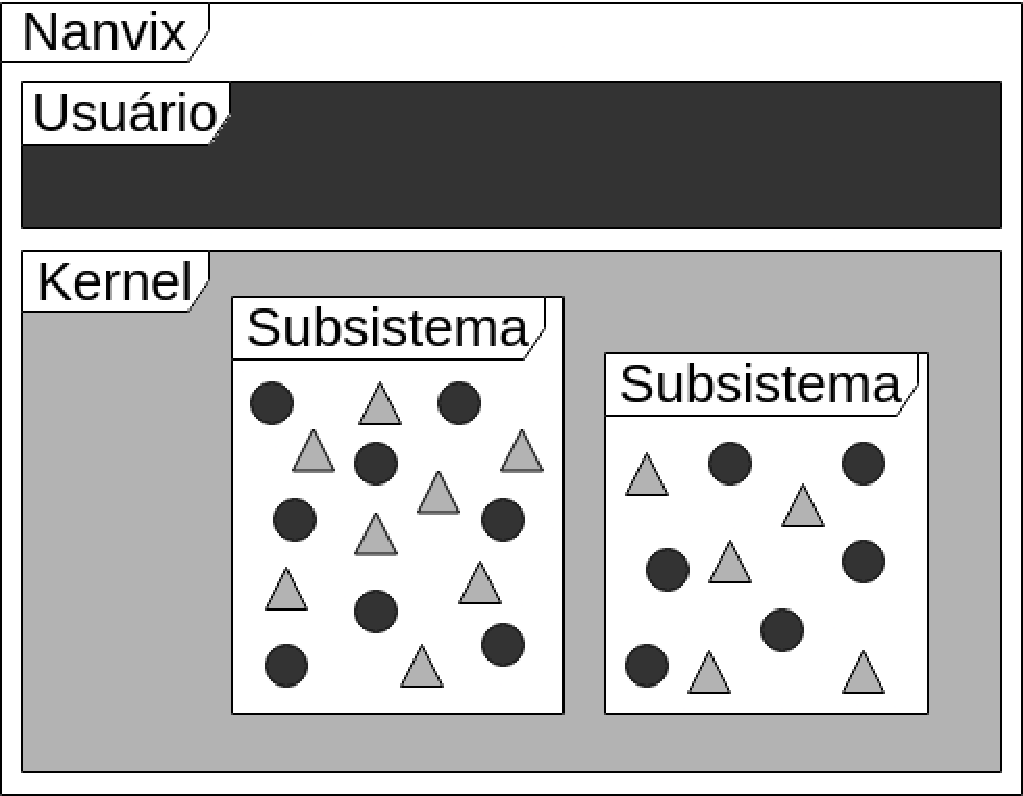
\includegraphics[width=\textwidth]{content/images/nanvix-without-uarea-uk.pdf}}
	\qquad
	\subcaptionminipage[fig.nanvix.with-uarea]
                   {.4\textwidth}
                   {\os com isolamento.}
                   {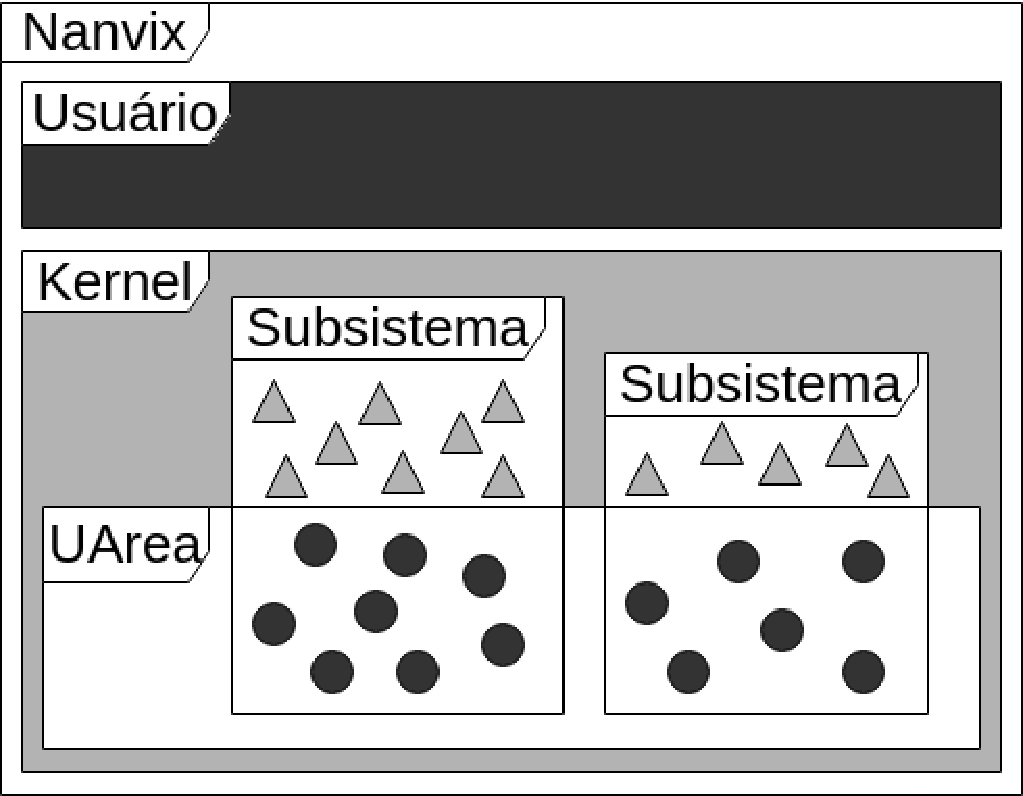
\includegraphics[width=\textwidth]{content/images/nanvix-with-uarea-uk.pdf}}

	
\includegraphics[width=.33\linewidth]{content/images/legenda.pdf}
	
	\caption{Diferença da estrutura do \nanvix com e sem a \textit{User Area}.}%
\end{figure}

\subsection{Isolamento do contexto de um processo de usuário}
\label{sec.dev.kernel-usuario}

\subsubsection{Divisão de Dados e Instruções}
\label{sec.divisao-dados-instrucao}

    Para a virtualização de processos através da conteinerização, é recomendável que as informações relevantes para a manipulação dos processos em execução estejam isoladas das informações internas do próprio \os para que os recursos de \hardware sejam utilizados de maneira eficiente~\cite{choudhary2017critical}.
    A \autoref{fig.nanvix.without-uarea} ilustra como os subsistemas do \nanvix são originalmente estruturados. Não há uma divisão explícita do que são dados para funcionamento interno do \os ou dependências locais do processo.
    Esta abordagem torna algumas das funcionalidades do \os onerosas porque ela dificulta o acesso às informações do processo e impacta partes independentes do sistema, \eg migração e segurança dos processos.

    Além disso, a geração original de um executável do \nanvix compila todos os níveis em bibliotecas estáticas (\hal, \microkernel, \libnanvix, \ulibc e \multikernel) e as junta com a aplicação do usuário de forma a misturar o que é \kernel do que é usuário.
    %
    Visando a separação das informações entre usuário e \kernel, nós adaptamos o \script de ligação original do \nanvix. Na nova versão, as seções .text, .data, .bss e .rodata dos arquivos binários compilados são renomeados, especificando qual camada de abstração tal arquivo pertence. Desta forma, é possível identificar dados e instruções de cada camada do \nanvix, assim como as informações do usuário. Sendo assim, são geradas seções .text, .data, .rodata e .bss específicas para o \kernel e usuário. Portanto, todas as informações de \kernel, alocadas nos endereços mais baixos da memória, são isoladas das informações de aplicação, alocadas nos endereços mais altos da memória. Neste processo, são exportadas algumas constantes que apontam onde começam e terminam as partes do binário que são relacionadas ao \kernel e à aplicação. Essas constantes permitem a manipulação e gerenciamento mais precisos dos segmentos de memória do \kernel e da aplicação.
    
    Através dessa estratégia, todos os \clusters passam a ter a mesma organização interna de \kernel, facilitando a migração. Ou seja, a migração pode ser feita através do salvamento dos dados e instruções da aplicação de um \cluster e restauração destes nas respectivas posições em outro \cluster. Essas posições são identificadas pelas constantes exportadas no processo de compilação. Com isso, evita-se manipulações mais complexas do processo como a busca em várias regiões de memória para montar o estado interno do processo.

    % \mytodo{colocar alguma parte do linker?}
    % \mytodo{Souto: ngm vai entender o código do linker mas seria legal colocar e discutir melhor sobre as constantes.}
    
\subsubsection{\textit{User Area}}
\label{sec.uarea}

    Além da separação de dados e instruções entre \kernel e aplicação, é necessário a identificação e separação das estruturas internas do \so que são manipuladas pelo usuário e constituem o estado interno do processo. Nesse contexto, é introduzido o conceito de conteinerização para isolar as dependências que o usuário possui dentro do \cluster. Ou seja, nós isolamos os dados que são gerenciados pelo \kernel mas pertencem ao contexto do processo de usuário. Neste contexto, nós isolamos tais dados em uma região de memória bem definida, denominada de \uarea. 

    Detalhadamente, a \uarea mantém informações sobre:
    \begin{enumerate}[label=(\roman*)]
        \item \Threads ativas, incluindo identificadores e contextos;
        \item Ponteiros para suas pilhas de execução; 
        \item Variáveis de controle e filas de escalonamento;
        \item Estruturas de gerenciamento de chamadas de sistema; e
        \item Estruturas de gerenciamento de memória (\eg sistema de paginação).
    \end{enumerate}

    Essa estrutura genérica foi projetada para englobar as várias arquiteturas suportadas pelo \nanvix. Além disso, a estrutura permite a modificação e expansão, não se limitando ao estado atual do desenvolvimento do \nanvix, para atender os objetivos de outros projetos que usufruam do \nanvix.

\section{Migração de Processos}
\label{sec.migracao}

Como aplicação direta do isolamento do processo, a migração de processos torna-se viável. Especificamente, nós eliminamos a necessidade de descobrir quais são e onde estão as informações que compõem o estado de um processo dentro do \nanvix através da criação de uma instância isolada do espaço do usuário via conteinerização, facilitando a transferência de seu contexto. Isso só é possível porque os \clusters possuem uma estrutura de \kernel idêntica (devido às mudanças desenvolvidas no processo de compilação detalhados na \autoref{sec.divisao-dados-instrucao}). Por este motivo, eliminamos o envio de dados redundantes entre \clusters referentes à instância local do \os, atenuando o impacto da migração sobre a \noc.

\subsection{Rotina de migração}
\label{sec.rotina-migracao}

Para a migração de um processo entre \clusters foi desenvolvida uma rotina de migração. A funcionalidade é similar ao \criu, ferramenta utilizada por \softwares de gerenciamento de contêineres como o Docker. Porém, a migração é executada por intermédio de \daemons do \os. Neste do projeto, implementamos o algoritmo \hotmigration para migração de processos. A técnica de \hotmigration migra a aplicação durante sua execução, copiando as páginas de memória e o estado de execução da aplicação e restaurando a aplicação depois da transferência completa dos dados. A seguir é detalhado o fluxo de execução da migração:

\begin{description}
	\item[1. Congelamento da execução do processo em um estado consistente.] \hfill
	
	Antes do envio da aplicação a outro \cluster, é necessário que o processo esteja em um estado consistente e estático. Isso significa que durante o processo de migração é preciso que todas as operações dele sejam pausadas. Isso é feito objetivando evitar inconsistências que podem ser causadas por condições de corrida \eg impedir perda de instruções, retornos de chamadas de sistemas, sinais de sincronização, etc. Para atingir esse estado consistente, a chamada de sistema \freeze é invocada. Esta é uma chamada de sistema que é tratada apenas pelo \mcore. Especificamente, esta chamada ativa uma variável interna do \so que impede o escalonamento de \threads de aplicação (\threads que não executam no \mcore) e envia um sinal de reescalonamento para todos os \scores, para que as \threads de usuário saiam de execução o mais rápido possível. Isso garante uma pausa na aplicação sem que o \so seja impedido de executar, o que é imprescindível para a migração, já que as informações do processo precisam ser enviadas pelas interfaces \noc do \cluster remetente, o que exige que o \so atenda às requisições de envio de dados. Após o travamento no escalonamento de \threads de usuário, novas chamadas de sistema requisitadas pela aplicação não podem ocorrer. Sendo assim, após a migração, o \cluster destinatário atenderá às chamadas não atendidas e reconhecerá as atendidas, pois as estruturas de sincronização e variáveis de retorno são migradas também durante o processo. Após o congelamento do escalonamento e a retirada das \threads de usuário dos \scores, o processo é considerado consistente e seu contexto está apto para ser migrado.

	\item[2. Transferência do contexto do processo entre \clusters.] \hfill
	
	Com o processo em um estado consistente, uma \task de sistema, que é executada no \mcore, é criada para o envio dos dados ao \cluster destinatário. Através das abstrações de comunicação \mailbox e \portal, as seções de dados e instruções do processo são enviadas ao \cluster destinatário. Logo após, a \uarea é enviada. O envio de dados, instruções e \uarea garantem que o contexto inteiro do processo seja enviado, possibilitando a retomada da execução no \cluster destinatário.

	\item[3. Restauração da execução do processo no \cluster destino.] \hfill
	
	Com o contexto do processo já no \cluster destinatário, a execução é restaurada. Isso é feito pela chamada de sistema \unfreeze, que descongela o escalonamento de \threads de usuário. Assim, a execução do processo continua normalmente, agora em outro \cluster.
\end{description}

\mytodo{detalhar como funcionam as tasks e threads em cada cluster: remetente e destinatario}
\mytodo{como funciona a migração para um cluster com nenhum processo alocado}